\documentclass[12pt,letterpaper]{article}
\usepackage{graphicx,textcomp}
\usepackage{natbib}
\usepackage{setspace}
\usepackage{fullpage}
\usepackage{color}
\usepackage[reqno]{amsmath}
\usepackage{amsthm}
\usepackage{fancyvrb}
\usepackage{amssymb,enumerate}
\usepackage[all]{xy}
\usepackage{endnotes}
\usepackage{lscape}
\newtheorem{com}{Comment}
\usepackage{float}
\usepackage{hyperref}
\newtheorem{lem} {Lemma}
\newtheorem{prop}{Proposition}
\newtheorem{thm}{Theorem}
\newtheorem{defn}{Definition}
\newtheorem{cor}{Corollary}
\newtheorem{obs}{Observation}
\usepackage[compact]{titlesec}
\usepackage{dcolumn}
\usepackage{tikz}
\usetikzlibrary{arrows}
\usepackage{multirow}
\usepackage{xcolor}
\newcolumntype{.}{D{.}{.}{-1}}
\newcolumntype{d}[1]{D{.}{.}{#1}}
\definecolor{light-gray}{gray}{0.65}
\usepackage{url}
\usepackage{listings}
\usepackage{color}

\definecolor{codegreen}{rgb}{0,0.6,0}
\definecolor{codegray}{rgb}{0.5,0.5,0.5}
\definecolor{codepurple}{rgb}{0.58,0,0.82}
\definecolor{backcolour}{rgb}{0.95,0.95,0.92}

\lstdefinestyle{mystyle}{
	backgroundcolor=\color{backcolour},   
	commentstyle=\color{codegreen},
	keywordstyle=\color{magenta},
	numberstyle=\tiny\color{codegray},
	stringstyle=\color{codepurple},
	basicstyle=\footnotesize,
	breakatwhitespace=false,         
	breaklines=true,                 
	captionpos=b,                    
	keepspaces=true,                 
	numbers=left,                    
	numbersep=5pt,                  
	showspaces=false,                
	showstringspaces=false,
	showtabs=false,                  
	tabsize=2
}
\lstset{style=mystyle}
\newcommand{\Sref}[1]{Section~\ref{#1}}
\newtheorem{hyp}{Hypothesis}

\title{Problem Set 3 - Answers}
\date{Due: November 19, 2022}
\author{Applied Stats/Quant Methods 1}
\author{Sara Cid}


\begin{document}
	\maketitle
	\section*{Instructions}
	\begin{itemize}
		\item Please show your work! You may lose points by simply writing in the answer. If the problem requires you to execute commands in \texttt{R}, please include the code you used to get your answers. Please also include the \texttt{.R} file that contains your code. If you are not sure if work needs to be shown for a particular problem, please ask.
	\item Your homework should be submitted electronically on GitHub.
	\item This problem set is due before 23:59 on Sunday November 19, 2023. No late assignments will be accepted.

	\end{itemize}

		\vspace{.25cm}
	
\noindent In this problem set, you will run several regressions and create an add variable plot (see the lecture slides) in \texttt{R} using the \texttt{incumbents\_subset.csv} dataset. Include all of your code.

\newpage

	\vspace{.5cm}
\section*{Question 1}
\vspace{.25cm}
\noindent We are interested in knowing how the difference in campaign spending between incumbent and challenger affects the incumbent's vote share. 
	\begin{enumerate}
		\item Run a regression where the outcome variable is \texttt{voteshare} and the explanatory variable is \texttt{difflog}. \vspace{0.25cm}
		
		Code for the regression: 
		\lstinputlisting[language=R, linerange={40-41}]{PS3_SC_answers.R} 
		
		Reporting regression results: 
		% Table created by stargazer v.5.2.3 by Marek Hlavac, Social Policy Institute. E-mail: marek.hlavac at gmail.com% Date and time: Thu, Nov 16, 2023 - 12:22:38
	\begin{table}[!htbp] \centering   \caption{Model 1 Regression Results}   \label{} \begin{tabular}{@{\extracolsep{5pt}}lc} \\[-1.8ex]\hline \hline \\[-1.8ex]  & \multicolumn{1}{c}{VoteSh} \\ \cline{2-2} \hline \\[-1.8ex]  DiffLog & 0.042$^{***}$ \\   & (0.001) \\   & \\  Constant & 0.579$^{***}$ \\   & (0.002) \\   & \\ \hline \\[-1.8ex] Observations & 3,193 \\ R$^{2}$ & 0.367 \\ Adjusted R$^{2}$ & 0.367 \\ \hline \hline \\[-1.8ex] \textit{Note:}  & \multicolumn{1}{r}{$^{*}$p$<$0.05; $^{**}$p$<$0.01; $^{***}$p$<$0.001} \\ \end{tabular} \end{table} 
		
		Brief interpretation: 
		The results show that a one-unit increase in difflog is associated, on average, with a 0.042 unit increase in voteshare (this is 4.2\% higher). Since p $<$ 0.001, we can reject the null hypothesis that there is no association between difflog and voteshare, or that the slope of difflog in this model is zero. 
		
		\item Make a scatterplot of the two variables and add the regression line. 	\vspace{0.25cm}
		
		Code for the scatterplot: 
		\lstinputlisting[language=R, linerange={49-57}]{PS3_SC_answers.R}
		
		Showing the scatterplot: 
		\begin{figure}[H]
			\centering
			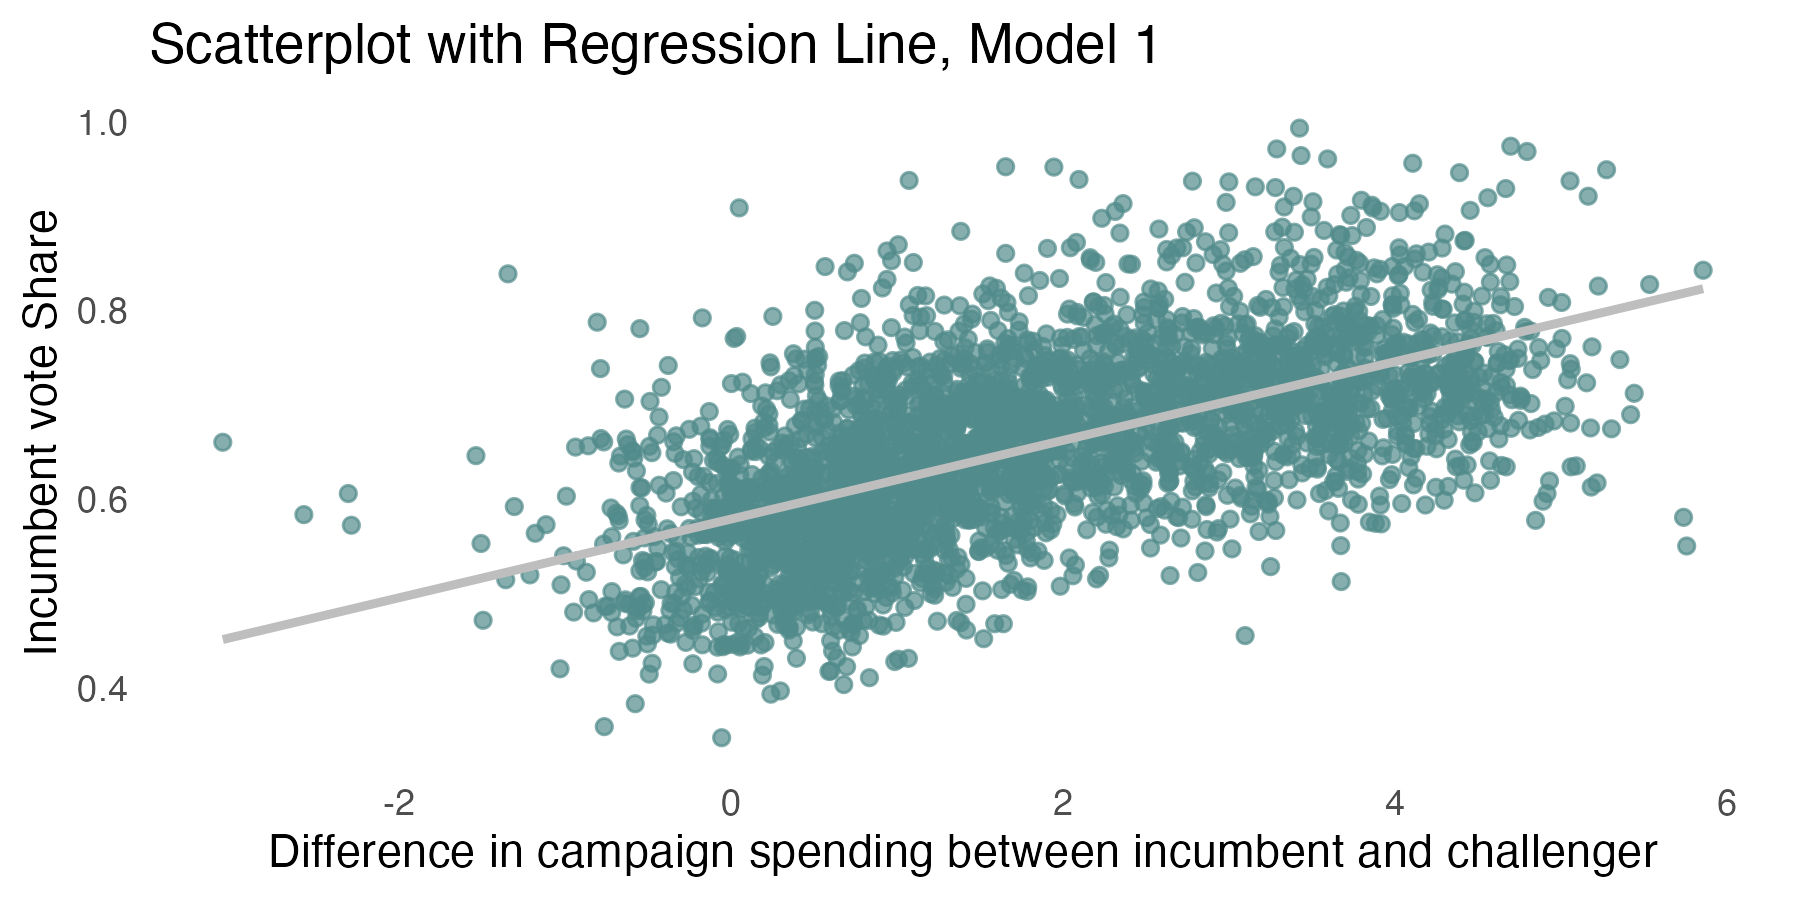
\includegraphics[width=0.8\textwidth]{/Users/sarabcidf/Desktop/ASDS/Statistics/StatsI_Fall2023/problemSets/PS03/my_answers/plot1.png}
			\caption{Model 1 Plot}
		\end{figure}
		
		Brief interpretation: 
		The scatterplot is consistent with the results from the regression, showing a positive association between DiffLog and VoteShare. The shape that forms from the points is consistent with this as well, although the plot shows a significant amount of noise. 
		
		\item Save the residuals of the model in a separate object.	
		
		Code for saving the residuals: 
		\lstinputlisting[language=R, linerange={46-47}]{PS3_SC_answers.R}
		
		\item Write the prediction equation.
		
		{\setlength{\abovedisplayskip}{2pt} 
			\setlength{\belowdisplayskip}{6pt} 
		
		\begin{flalign*}
			&\text{VoteSh} = 0.579 + 0.042 \cdot \text{DiffLog}  &
		\end{flalign*}
		
			where:  $VoteSh$: Incumbent's vote share , and $DiffLog$: Logarithm of the difference between incumbent and challenger's spending
	   }
		
 		\end{enumerate}
	
\newpage

\section*{Question 2}
\noindent We are interested in knowing how the difference between incumbent and challenger's spending and the vote share of the presidential candidate of the incumbent's party are related.	\vspace{.25cm}
	\begin{enumerate}
		\item Run a regression where the outcome variable is \texttt{presvote} and the explanatory variable is \texttt{difflog}. \vspace{0.25cm}
		
		Code for the regression:
		\lstinputlisting[language=R, linerange={82-84}]{PS3_SC_answers.R}
		
		Reporting regression results:  
		% Table created by stargazer v.5.2.3 by Marek Hlavac, Social Policy Institute. E-mail: marek.hlavac at gmail.com% Date and time: Thu, Nov 16, 2023 - 12:31:45
		\begin{table}[!htbp] \centering   \caption{Model 2 Regression Results}   \label{} \begin{tabular}{@{\extracolsep{5pt}}lc} \\[-1.8ex]\hline \hline \\[-1.8ex]  & \multicolumn{1}{c}{PresVote} \\ \cline{2-2} \hline \\[-1.8ex]  DiffLog & 0.024$^{***}$ \\   & (0.001) \\   & \\  Constant & 0.508$^{***}$ \\   & (0.003) \\   & \\ \hline \\[-1.8ex] Observations & 3,193 \\ R$^{2}$ & 0.088 \\ Adjusted R$^{2}$ & 0.088 \\ \hline \hline \\[-1.8ex] \textit{Note:}  & \multicolumn{1}{r}{$^{*}$p$<$0.05; $^{**}$p$<$0.01; $^{***}$p$<$0.001} \\ \end{tabular} \end{table} 
		
		Brief interpretation: 
		The results show that a one-unit increase in difflog is associated, on average, with a 0.024 unit increase in presvote (this is 2.4\% higher). Since p $<$ 0.001, we can reject the null hypothesis that there is no association between difflog and presvote, or that the slope of difflog in this model is zero. 
		
		\item Make a scatterplot of the two variables and add the regression line. \vspace{0.25cm}
		
		Code for the scatterplot: 
		\lstinputlisting[language=R, linerange={89-97}]{PS3_SC_answers.R}
		
		Showing the scatterplot: 
		\begin{figure}[H]
			\centering
			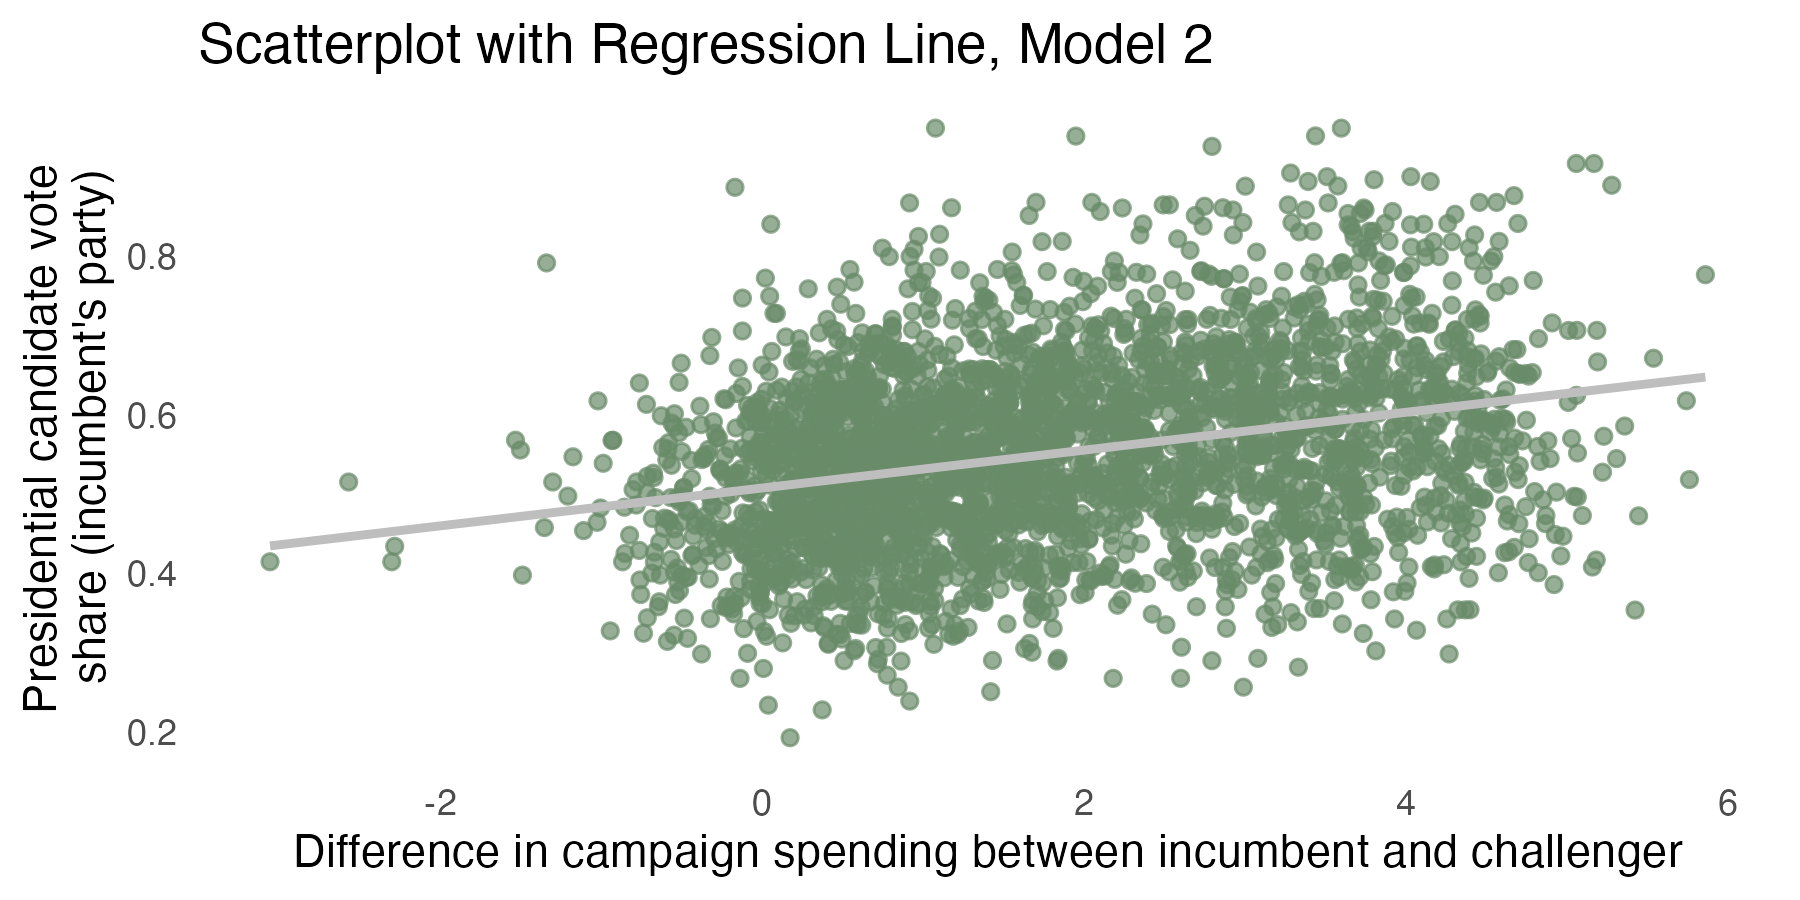
\includegraphics[width=0.8\textwidth]{/Users/sarabcidf/Desktop/ASDS/Statistics/StatsI_Fall2023/problemSets/PS03/my_answers/plot2.png}
			\caption{Model 2 Plot}
		\end{figure}
		
		Brief interpretation: 
		Again, the scatterplot is consistent with the results from the regression, this time showing a positive association between DiffLog and PresVote. The shape that forms from the points is consistent with this as well, although this plot shows a considerable amount of noise (more than in the first one).
		
		\item Save the residuals of the model in a separate object.	\vspace{0.25cm}
		
		Code for saving the residuals: 
		\lstinputlisting[language=R, linerange={86-87}]{PS3_SC_answers.R}
		
		\item Write the prediction equation.
		
		{\setlength{\abovedisplayskip}{2pt} 
			\setlength{\belowdisplayskip}{6pt} 
			
			\begin{flalign*}
				&\text{PresVote} = 0.508 + 0.024 \cdot \text{DiffLog}  &
			\end{flalign*}
			
			where $PresSh$: Vote share of the presidential candidate of the incumbent's party, and $DiffLog$: Logarithm of the difference between incumbent and challenger's spending
		} 
		
	\end{enumerate}
	
	\newpage	
\section*{Question 3}

\noindent We are interested in knowing how the vote share of the presidential candidate of the incumbent's party is associated with the incumbent's electoral success.
	\vspace{.25cm}
	\begin{enumerate}
		\item Run a regression where the outcome variable is \texttt{voteshare} and the explanatory variable is \texttt{presvote}. \vspace{.25cm}
		
		Code for the regression: 	
		\lstinputlisting[language=R, linerange={119-121}]{PS3_SC_answers.R}
		
		Reporting regression results: 
		% Table created by stargazer v.5.2.3 by Marek Hlavac, Social Policy Institute. E-mail: marek.hlavac at gmail.com% Date and time: Thu, Nov 16, 2023 - 12:33:52
		\begin{table}[!htbp] \centering   \caption{Model 3 Regression Results}   \label{} \begin{tabular}{@{\extracolsep{5pt}}lc} \\[-1.8ex]\hline \hline \\[-1.8ex]  & \multicolumn{1}{c}{VoteSh} \\ \cline{2-2} \hline \\[-1.8ex]  PresVote & 0.388$^{***}$ \\   & (0.013) \\   & \\  Constant & 0.441$^{***}$ \\   & (0.008) \\   & \\ \hline \\[-1.8ex] Observations & 3,193 \\ R$^{2}$ & 0.206 \\ Adjusted R$^{2}$ & 0.206 \\ \hline \hline \\[-1.8ex] \textit{Note:}  & \multicolumn{1}{r}{$^{*}$p$<$0.05; $^{**}$p$<$0.01; $^{***}$p$<$0.001} \\ \end{tabular} \end{table} 
		
		Brief interpretation: 
		The results show that a one-unit increase in presvote is associated, on average, with a 0.388 unit increase in voteshare (this is 38.8\% higher). The coefficient is very large in magnitude. Since p $<$ 0.001, we can reject the null hypothesis that there is no association between presvote and voteshare, or that the slope of presvote in this model is zero. 
			
		\item Make a scatterplot of the two variables and add the regression line. \vspace{.25cm}
		
		Code for the scatterplot: 
		\lstinputlisting[language=R, linerange={123-131}]{PS3_SC_answers.R}
		
		Showing the scatterplot: 
		\begin{figure}[H]
			\centering
			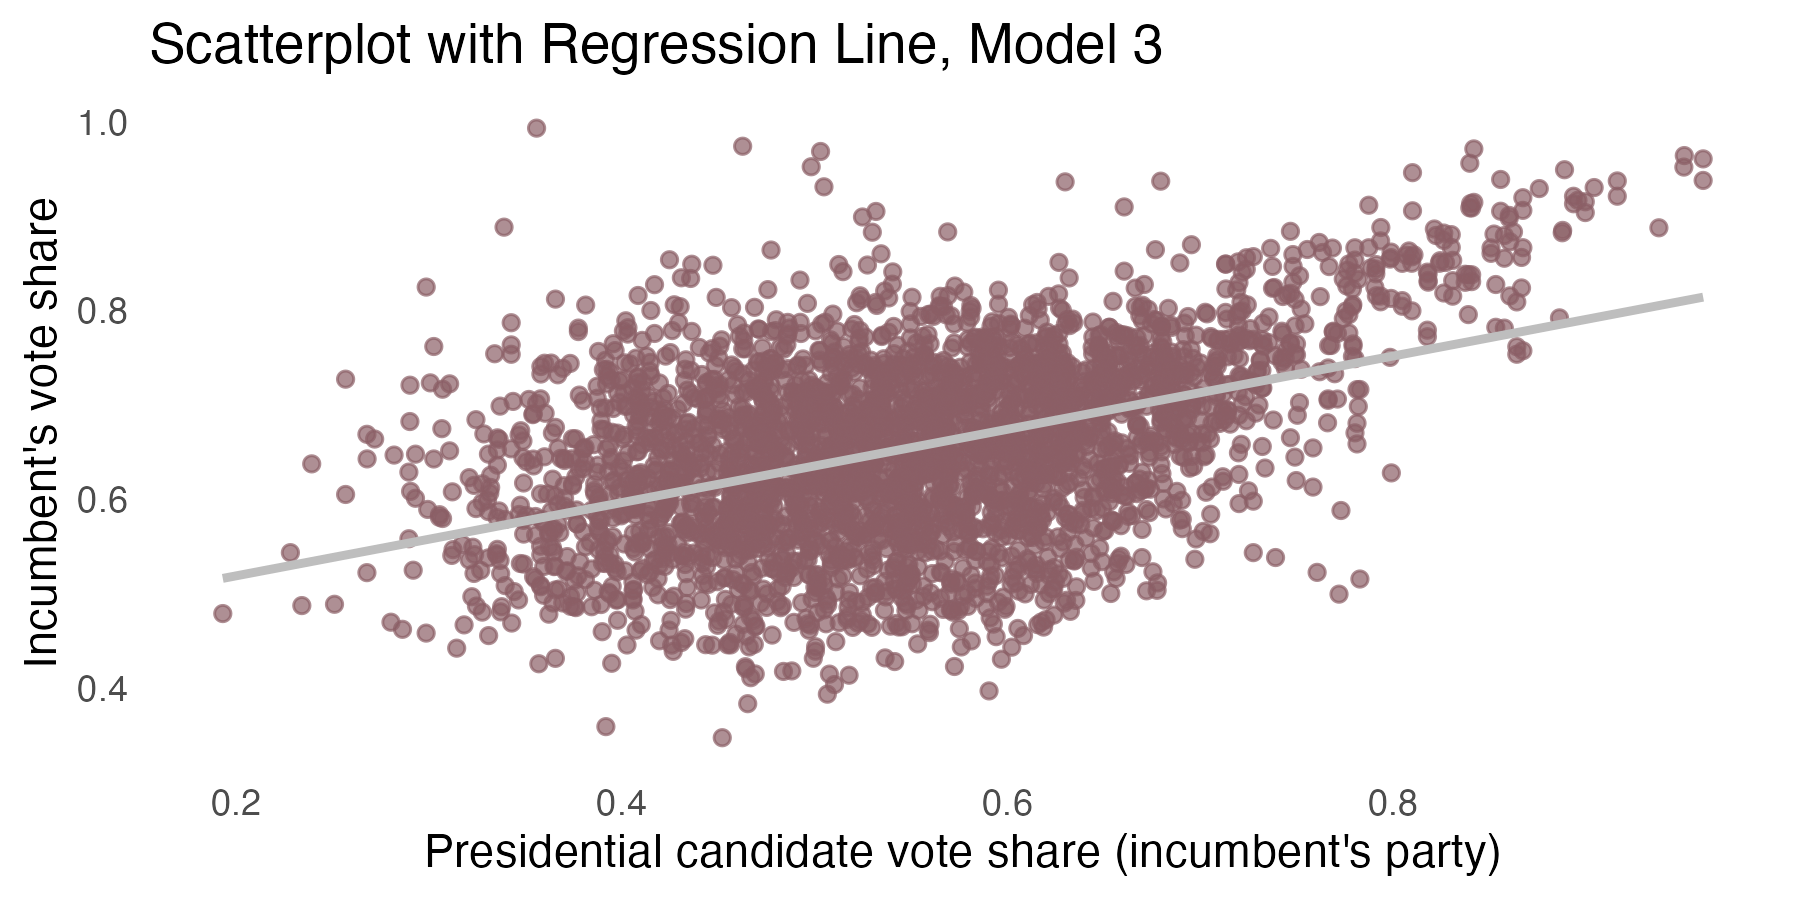
\includegraphics[width=0.8\textwidth]{/Users/sarabcidf/Desktop/ASDS/Statistics/StatsI_Fall2023/problemSets/PS03/my_answers/plot3.png}
			\caption{Model 3 Plot}
		\end{figure}
		
		Brief interpretation: 
		Again, the scatterplot is consistent with the results from the regression, this time showing a positive association between PresVote and VoteShare. The shape that forms from the points is consistent with this as well, although there is a significant amount of noise once again. 
			
		\item Write the prediction equation.
		
		{\setlength{\abovedisplayskip}{2pt} 
			\setlength{\belowdisplayskip}{6pt} 
			
			\begin{flalign*}
				&\text{VoteSh} = 0.441 + 0.388 \cdot \text{PresVote}  &
			\end{flalign*}
			
			where: 
			
			\begin{itemize}
				\item $VoteSh$: Incumbent's vote share
				\item $PresVote$: Vote share of the presidential candidate of the incumbent's party
			\end{itemize}
		}
		
	\end{enumerate}
	

\newpage	
\section*{Question 4}

\noindent The residuals from part (a) tell us how much of the variation in \texttt{voteshare} is $not$ explained by the difference in spending between incumbent and challenger. The residuals in part (b) tell us how much of the variation in \texttt{presvote} is $not$ explained by the difference in spending between incumbent and challenger in the district.
	\begin{enumerate}
		\item Run a regression where the outcome variable is the residuals from Question 1 and the explanatory variable is the residuals from Question 2.	\vspace{.25cm}
		
		Code for the regression: 
		\lstinputlisting[language=R, linerange={153-155}]{PS3_SC_answers.R}
		
		Reporting the regression results: 
		% Table created by stargazer v.5.2.3 by Marek Hlavac, Social Policy Institute. E-mail: marek.hlavac at gmail.com% Date and time: Thu, Nov 16, 2023 - 12:42:08
		\begin{table}[!htbp] \centering   \caption{Model 4 Regression Results}   \label{} \begin{tabular}{@{\extracolsep{5pt}}lc} \\[-1.8ex]\hline \hline \\[-1.8ex]  & \multicolumn{1}{c}{Model1Res} \\ \cline{2-2} \hline \\[-1.8ex]  Model2Res & 0.257$^{***}$ \\   & (0.012) \\   & \\  Constant & $-$0.000 \\   & (0.001) \\   & \\ \hline \\[-1.8ex] Observations & 3,193 \\ R$^{2}$ & 0.130 \\ Adjusted R$^{2}$ & 0.130 \\ \hline \hline \\[-1.8ex] \textit{Note:}  & \multicolumn{1}{r}{$^{*}$p$<$0.05; $^{**}$p$<$0.01; $^{***}$p$<$0.001} \\ \end{tabular} \end{table} 
		
		Brief interpretation: 
		The results show that a one-unit increase in Model2Res is associated, on average, with a 0.257 unit increase in Model1Res. Since p $<$ 0.001, we can reject the null hypothesis that there is no association between Model2Res and Model1Res, or that the slope of Model2Res in this model is zero. 
		
		\item Make a scatterplot of the two residuals and add the regression line. 	\vspace{.25cm}
		
		Code for the scatterplot: 
		\lstinputlisting[language=R, linerange={157-165}]{PS3_SC_answers.R}
		
		Showing the scatterplot: 
		\begin{figure}[H]
			\centering
			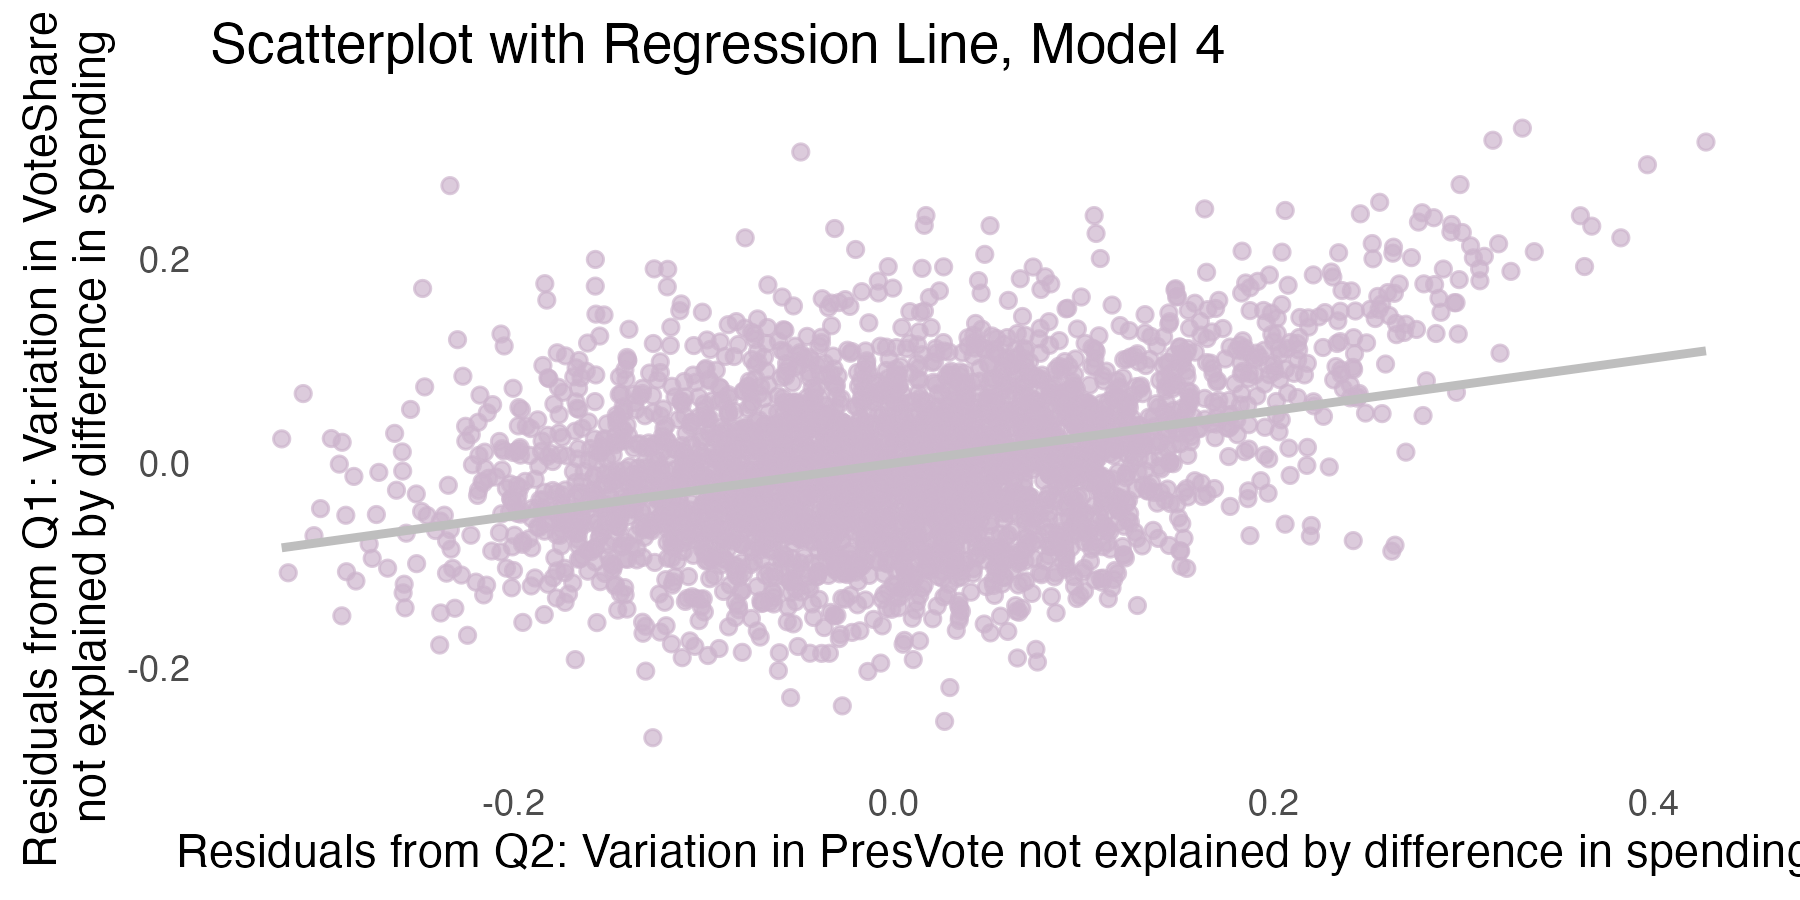
\includegraphics[width=0.8\textwidth]{/Users/sarabcidf/Desktop/ASDS/Statistics/StatsI_Fall2023/problemSets/PS03/my_answers/plot4.png}
			\caption{Model 4 Plot}
		\end{figure}
		
		Brief interpretation: 
		Once more, the scatterplot is consistent with the results from the regression, this time showing a positive association between the residuals from Model2 and those of Model1. The shape that forms from the points is consistent with this as well, although there is a significant amount of noise. 
		
		\item Write the prediction equation.
		
		{\setlength{\abovedisplayskip}{2pt} 
			\setlength{\belowdisplayskip}{6pt} 
			
			\begin{flalign*}
				&\text{Resid1} = 0 + 0.257 \cdot \text{Resid2}  &
			\end{flalign*}
			
			where: 
			
			\begin{itemize}
				\item $Resid1$: Residuals from first model (variation in incumbent's vote share not explained by difference in spending)
				\item $Resid2$: Residuals from second model (variation in presidential candidate's vote share not explained by difference in spending)
			\end{itemize}
		}
		
	\end{enumerate}
	
	\newpage	

\section*{Question 5}
\noindent What if the incumbent's vote share is affected by both the president's popularity and the difference in spending between incumbent and challenger? 
	\begin{enumerate}
		\item Run a regression where the outcome variable is the incumbent's \texttt{voteshare} and the explanatory variables are \texttt{difflog} and \texttt{presvote}.	\vspace{.25cm}
		
		Code for the regression: 
		\lstinputlisting[language=R, linerange={187-189}]{PS3_SC_answers.R}
		
		Reporting regression results: 
		% Table created by stargazer v.5.2.3 by Marek Hlavac, Social Policy Institute. E-mail: marek.hlavac at gmail.com% Date and time: Thu, Nov 16, 2023 - 12:36:14
		\begin{table}[!htbp] \centering   \caption{Model 5 Regression Results}   \label{} \begin{tabular}{@{\extracolsep{5pt}}lc} \\[-1.8ex]\hline \hline \\[-1.8ex]  & \multicolumn{1}{c}{VoteSh} \\ \cline{2-2} \hline \\[-1.8ex]  DiffLog & 0.036$^{***}$ \\   & (0.001) \\   & \\  PresVote & 0.257$^{***}$ \\   & (0.012) \\   & \\  Constant & 0.449$^{***}$ \\   & (0.006) \\   & \\ \hline \\[-1.8ex] Observations & 3,193 \\ R$^{2}$ & 0.450 \\ Adjusted R$^{2}$ & 0.449 \\ \hline \hline \\[-1.8ex] \textit{Note:}  & \multicolumn{1}{r}{$^{*}$p$<$0.05; $^{**}$p$<$0.01; $^{***}$p$<$0.001} \\ \end{tabular} \end{table} 
		
		Brief interpretation: 
		The results show that a one-unit increase in difflog is associated, on average and holding presvote constant, with a 0.036 unit increase in voteshare. Since p $<$ 0.001, we can reject the null hypothesis that there is no association between difflog and voteshare, or that the slope of difflog in this model is zero. 
		For presvote, the results show that a one-unit increase in presvote is associated, on average and holding difflog constant, with a 0.257 unit increase in voteshare. Since p $<$ 0.001, we can reject the null hypothesis that there is no association between presvote and voteshare, or that the slope of difflog in this model is zero. 
		In comparison with Model 1 and Model 2, where we tested the association of difflog and voteshare, and then presvote and voteshare separately, the coefficients in this last model are slightly smaller. This is explained by the fact that presvote and difflog share some variability among each other, which we also proved in Model 3. 
		
		\item Write the prediction equation. 
		
		{\setlength{\abovedisplayskip}{2pt} 
			\setlength{\belowdisplayskip}{6pt} 
			
			\begin{flalign*}
				&\text{VoteSh} = 0.449 + 0.036 \cdot \text{DiffLog} + 0.257 \cdot \text{PresVote} &
			\end{flalign*}
			
			where: 
			
			\begin{itemize}
				\item $VoteSh$: Incumbent's vote share
				\item $DiffLog$: Logarithm of the difference between incumbent and challenger's spending
				\item $PresVote$: Vote share of the presidential candidate of the incumbent's party
			\end{itemize}
		}
		
		\item What is it in this output that is identical to the output in Question 4? Why do you think this is the case? \vspace{.25cm}
		
		Code to compare residuals: 
		\lstinputlisting[language=R, linerange={204-229}]{PS3_SC_answers.R}
		
		First, the coefficient for presvote in Model 5 is the same as that of Resid2 in Model 4. This is because both coefficients describe the relationship between the unexplained variation in presvote and the unexplained variation in voteshare after accounting for difflog. 
		
		In Model 4, the coefficient of Resid2 describes the relationship between the unexplained variation in presvote after accounting for difflog (Resid2) and the unexplained variation in voteshare after accounting for difflog (Resid1) because we are running a regression of Resid1 over Resid2. 
	
		In Model 5, the coefficient of presvote captures essentially the same thing: how presvote varies with share, after accounting for difflog, which is the other independent variable in the multivariate model. 
		
		Also, the residuals in Models 4 and 5 are the same, because since our outcome in Model 4 is the unexplained variation in voteshare after including difflog in our regression, and since our explanatory variable in Model 4 is the unexplained variation in presvote after including difflog in our regression, the residuals of this model are exactly the same thing as the residuals in Model 5, where we run a multivariate regression of voteshare over difflog and presvote. 
	
		That is, the residuals in both cases consist of the unexplained variation in voteshare after accounting for both difflog and presvote. 
		
	\end{enumerate}




\end{document}
